\sect{LLM-Guided Robotics Applications in Industrial and Laboratory Environments}{roboticapplications}

Integrating LLMs into collaborative autonomous environments represents a key advance in automating complex experimental and manufacturing workflows. Unlike traditional SDLs and collaborative robotics systems based on fixed task sequences and domain-specific control scripts, LLMs can serve as high-level planners that translate abstract objectives into structured task protocols and dynamically adapt to new constraints \cite{yoshikawa2023large, kitchin2025evolving, xie2025toward, ruehle2025workflow}. In industry, \emph{Fan et al.} \cite{fan2025embodied} implemented GPT-4-based embodied manufacturing intelligence for autonomous toolpath generation, \emph{Wang et al.} \cite{wang2024llm} demonstrated vision-language navigation for Automated Guided Vehicles (AGVs), and \emph{Gkournelos et al.} \cite{gkournelos2024llm} combined Digital Twins with behavior-based planning for collaborative assembly. Collectively, these works show LLMs evolving from passive code generators to reasoning agents coordinating autonomous systems across laboratories and factories, improving adaptability, safety, and accessibility in automation.


At the core of LLM-guided collaborative autonomy lies the ability to translate unstructured NL into machine-interpretable commands consistent with experimental constraints and system capabilities. The \emph{CLAIRify} framework \cite{yoshikawa2023large} achieves this via an iterative prompt-verification loop enforcing the syntax and semantics of a domain-specific chemistry language (XDL) before dispatching validated task graphs to a TAMP pipeline solved with PDDLStream, ensuring semantic and physical feasibility. Similar principles appear in manufacturing, where LLMs extract process parameters, select end-effectors, and generate verified toolpaths with reflection modules \cite{fan2025embodied}; in assembly, where dual-agent architectures separate dialogue handling from instruction translation, yielding executable schedules verified through behavior trees \cite{gkournelos2024llm}; and in navigation, where operator instructions are grounded in 3D semantic maps to produce path-planning code for Automated Guided Vehicles \cite{wang2024llm}. Together, these systems show how LLMs decompose abstract objectives into verifiable sub-goals grounded in domain knowledge and multimodal perception, enabling adaptive and safe autonomy in collaborative robotic environments.

From an infrastructure perspective, \emph{Tom et al.} \cite{tom2024self} classify SDLs along two orthogonal dimensions of software and hardware autonomy, with LLM-guided robotic systems representing a key enabler for achieving Level 4 and potentially Level 5 autonomy, as illustrated in Figure~\ref{fig:placeholder}. In these systems, LLMs extend software autonomy by enabling closed-loop experimental workflows, including hypothesis formulation, code generation, and parameter optimization without direct human input \cite{tom2024self}. The autonomous agent loop proposed by \emph{Xie et al.} \cite{xie2025toward} exemplifies a transitional architecture toward higher autonomy, in which an LLM iteratively performs code synthesis, execution, and self-correction until experimental objectives are met. Comparable strategies have also been implemented in manufacturing, where LLM-based agents perform task decomposition and reflection-driven error recovery to achieve embodied intelligence in robotic processes \cite{fan2025embodied}. Hardware autonomy is simultaneously advancing through the integration of Digital Twins for collaborative assembly \cite{gkournelos2024llm} and mobile AGVs employing vision-and-language navigation on dynamic shop floors \cite{wang2024llm}. The interplay between these software and hardware layers defines the architecture of next-generation collaborative autonomous environments, supporting multi-domain workflows without extensive reconfiguration or task-specific programming \cite{tom2024self}.

\begin{figure}[H]
    \centering
    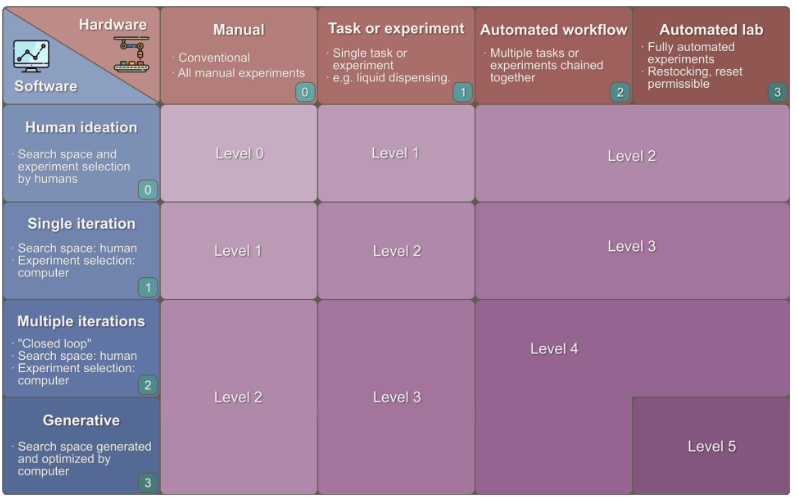
\includegraphics[width=1\linewidth]{Images/Schematic for the autonomy levels of SDLs based on the category of hardware and software autonomy achieved.png}
    \caption{Schematic for the autonomy levels of SDLs based on the category of hardware and software autonomy achieved \cite{tom2024self}}
    \label{fig:placeholder}
\end{figure}

Complementary studies by \emph{Ruehle et~al.} \cite{ruehle2025workflow,ruehle2025nano} advanced the formalisation of experimental workflows in SDLs through semantic representations and autonomous execution. The first work introduces a framework translating natural-language procedures into graph-based, machine-executable workflows with automatic validation and reproducibility control. The second demonstrates a fully automated SDL integrating robotic synthesis, in-line analysis, and closed-loop optimisation for nano- and advanced materials. These developments establish a direct link between semantic workflow management and autonomous experimentation, reinforcing the methodological foundation for scalable and reproducible SDL architectures.

Despite their promise, current LLM-guided autonomous systems face persistent challenges in reproducibility, safety assurance, latency, and domain adaptation. Key limitations include model hallucination, incomplete grounding in laboratory ontologies, and brittleness in zero-shot code generation, all of which constrain full autonomous deployment. Achieving real-time control remains difficult, as most systems still generate complete executable scripts rather than structured, parameterized commands, limiting adaptability to unforeseen conditions \cite{xie2025toward}. Similar vulnerabilities are observed in manufacturing, where LLM-driven agents may produce erroneous toolpaths or unsafe task allocations without embedded verification \cite{fan2025embodied,gkournelos2024llm}, and in navigation, where inadequate grounding can cause misinterpretation of operator instructions or semantic maps in dynamic environments \cite{wang2024llm}. 

A more resilient design would separate reasoning from execution, allowing the LLM to output machine-interpretable parameters that are passed to a validated translation layer, thereby enhancing operational safety and robustness. Until such architectures become standard, sandboxed code evaluation, strict protocol compliance, and local model deployment remain essential safeguards for data-sensitive or safety-critical settings. Existing mitigation approaches include in-context constraint injection \cite{yoshikawa2023large}, rule-based and programmatic verification \cite{kitchin2025evolving,yoshikawa2023large}, retrieval-augmented grounding \cite{boiko2023autonomous}, and modular fallback mechanisms incorporating human oversight \cite{tom2024self}. 

Progress beyond these constraints will depend on the development of standardized, machine-interpretable ontologies, richer multimodal grounding (e.g., vision, force sensing, spectroscopy), and the integration of safety-aware planning frameworks directly within the LLM-agent control loop. These advancements are essential for the transition from prototype platforms such as \emph{Claude-Light} and \emph{Coscientist} to industrial-scale, general-purpose collaborative environments capable of autonomous, reliable, and reproducible operation \cite{yoshikawa2023large}.

